
The accumulation of large-scale phylogenomic data sets leads to new challenges of comparison and visualisation of
distinct gene families, as well as of detecting the influence of each genomic region into the overall phylogenomic
signals. 
State-of-the-art phylogenetic methods take gene trees as input, and model the incongruence among them in
various ways, based on various assumptions. 
Many of these methods require the input gene trees to have at most one
representative from each species (e.g. by requiring the user to first run an orthology inference pipeline). This
limitation is hard to circumvent since almost all tree distance measures (required to measure incongruence between two
trees) assume that the same leaves are present on both trees.

There has been several attempts at describing phylogenetic trees as vectors of features, suitable for statistical
comparison, such as (Leigh et al. 2011, 2008; Susko et al. 2006; Narechania et al. 2016; Nye 2011; Yoshida, Fukumizu,
and Vogiatzis 2015; Lewitus and Morlon 2015; Kendall and Colijn 2016; Colijn and Plazzotta 2018) There are also a few
methods that rely on pairwise tree distance matrices, which could then be projected into a new coordinate system.

Unsupervised learning algorithms accept one of two forms of input: a design (also called feature) matrix X of size nXp
(n samples with p dimensions each), or a dissimilarity matrix D of size nXn describing the distances between each pair
of samples. Given D, one can project the samples into a feature space for further analysis (using multidimensional
scaling, for instance). However, this projection needs to be recalculated if new samples arise. Our method, on the other
hand, allows for disentangling the acquisition of sample gene trees and their projection, since their feature space can
be described without resorting to the whole set of existing sample trees. This can become particularly relevant when the
number of sample gene trees exceeds largely the number of reference species trees.

Visualisation and comparison of gene trees has been increasingly recognised as a way to objectively partition
phylogenetic signal and to detect potential sources of heterogeneity (Gori et al. 2016; Jombart et al. 2017; Huang et
al. 2016). So far all these methods rely on pairwise tree distance matrices, which implies that only uniquely labelled
trees can be compared (with the potential exception of (Kendall, Eldholm, and Colijn 2018) ). However in many cases we
cannot or prefer not to decide beforehand the orthologous groups. In these cases we must work with  the so-called
multi-labelled trees (or mul-trees, for short), which are trees with potentially more than one leaf with same label
(labelled by the same species, in our case). At the same time, dissimilarity matrices are not the only input for
classification algorithms, and describing samples through a coordinate system can have advantages.

There are many new algos thanks to big data, and our data sets are also increasing, therefore we can make use of their
novelties if we write our problem as a big data one. <...> This analysis can also help in ‘gene shopping’, i.e. when
only genomic regions with desired properties are selected (Smith, Brown, and Walker 2018). On the other hand, we might
be concerned if a certain selection of genes can be responsible for a bias in the results.

Each gene family tree is represented by a set of features, and may contain paralogs or missing species. Each gene family
can be represented by several trees, all sharing same pattern of missing/duplicate species, as in Bayesian posterior
distributions. (However for testing purposes we might prune individual trees from a gene family.)

A “gene family” and a “cluster” will usually be used interchangeably, although we know that several gene families with
their sets of trees may cluster together etc. The term “cluster” will be preferred for the resulting statistic or
observation in general, and not to the underlying process it tries to capture. “gene family” will be used to a set of
trees that should always be clustered together (never be split between clusters).

The features are distance measures to a set of common, full reference trees. The reference trees are species trees, and
are full (or complete) in the sense that must have all species under analysis (even if missing from some gene family).

The selection of ‘reference’ species trees follow the same rationale behind centroidQR (Jeon, Park, and Rosen 2001;
Park, Jeon, and Ben Rosen 2003), pivot-based indexing, or landmark-based manifolds in machine learning: instead of
comparing all gene family trees with each other using a predefined tree distance, we first compare them to a potentially
smaller number of ‘landmark’ (species) trees. However there is an important difference: in our case there may be very
few, if any, dissimilarities that can be calculated between arbitrary gene family trees with several leaves with same
species label (e.g. paralogs), or with no species in common. On the other hand there are several tree distances
available that can cope with gene-species tree pairs – and the species trees should have all species present.

If we are only interested in a few alternative hypothesis, let’s say a particular branch/node, then most distances fail
since they give equal weight to all distances (since we compare gene trees directly). OTOH by using anchoring sptrees we
can "weight" these hypotheses by their representativity in the reference sptrees (minimal case is to use just two
sptrees, as "only" dimensions in the eigenbasis).

At the same time, choosing just "a few" sptrees allows our matrix to be lower dimensional than a full pairwise distance.
This becomes more evident when 1) gene families are much larger than sptrees (more leaves), and 2) many samples from
many genefams are analysed (e.g. 1M trees per family).

The idea is that although we may lose a lot of resolution when comparing two gene family trees directly (assuming such
comparison can be accomplished), we may have higher resolution [signal] by comparing each gene family to a species tree.
The difference lies in the number of species in common: when comparing two gene families G1 and G2 representing
respectively n1 and n2 species (over possibly N species), they will have in the worst case only max(0,n1+n2-N) ≤
min(n1,n2)  ---  where min(n1,n2) is the worst case comparison between G1 or G2 and the species tree.


\begin{figure}[!htbp]
\begin{minipage}{7in}\centering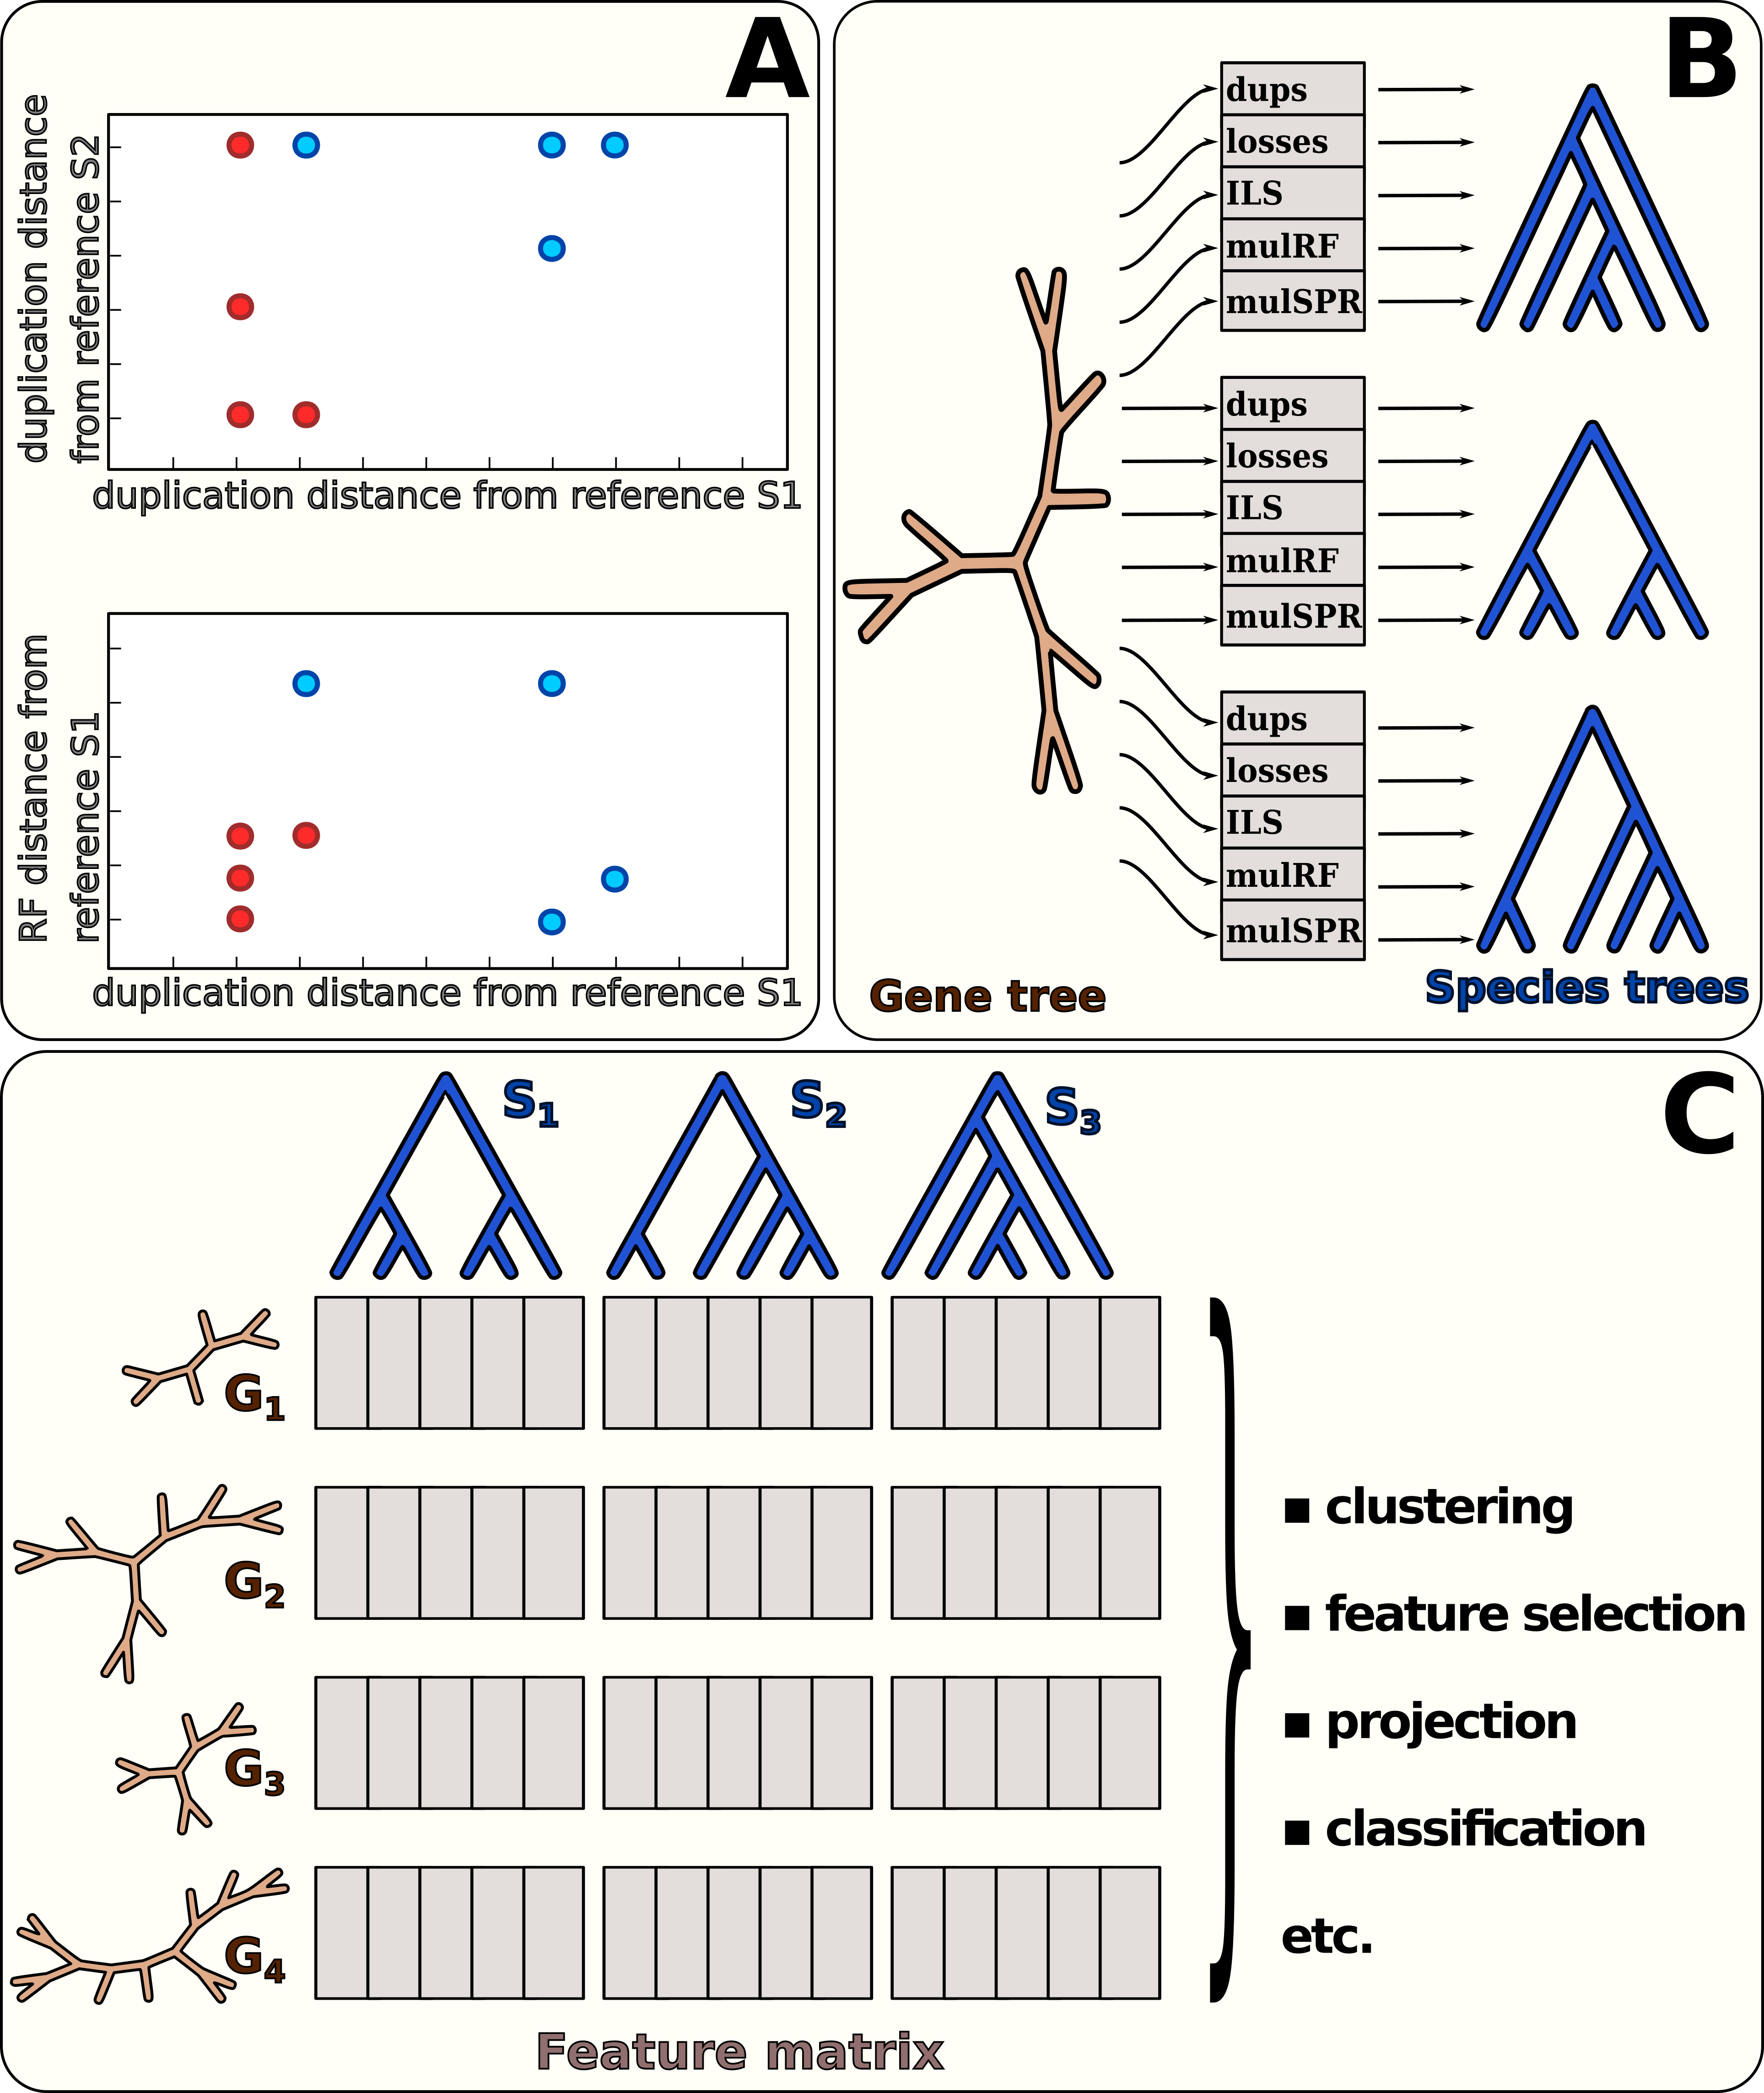
\includegraphics[width = 6.5in]{figure001.png}\end{minipage}
\caption{\label{figure01}
Schematic representation of the tree signal calculation. In panel A we show two simple cases for a sample of 8 gene
family trees: at the top we compare each gene tree to two distinct reference (species) trees using the minimum number of
duplications (duplication distance), and at the bottom we compare all sample gene trees to a single reference tree, but
using two distinct metrics --- the Robinson-Foulds (RF) distance and the duplication distance. Both comparisons provide
little information in isolation, but when combined allow for distinguishing the two groups of gene families (represented
by distinct colours). Panel B shows how the tree signal of a single gene family tree can be calculated, given a set of
species trees and a set of distances. Notice that currently we work with unrooted gene trees and rooted species trees.
In panel C we show that once we have the tree signal from each gene family, then we can create a feature matrix (‘design
matrix’) which can be used in downstream analyses.
}\end{figure}


